\chapter{Kiến thức cơ sở}
\label{chap:background}

Chương 2 sẽ trình bày các kiến thức cơ sở về ngôn ngữ lập trình Rust, cơ chế quản lý bộ nhớ hiệu quả và tính hướng hàm tạo nên đặc trưng của Rust.
Chương này cũng sẽ trình bày về các dạng biểu diễn của mã nguồn bao gồm cây AST, đồ thị CFG, đồ thị PDG và đồ thị CPG.
Joern, một bộ công cụ phân tích mã nguồn tĩnh, và những ưu điểm mà nó mang lại sẽ được nhắc tới ở phần cuối của chương.

\section{Ngôn ngữ lập trình Rust}

\subsection{Giới thiệu tổng quan}

% Rust was first introduced in 2006 by the Mozilla Foundation with its version 1.0 release announced in 2015. The language has since been adopted rapidly, with its strong focus on code safety and high performance comparable to that of C or C++ as the main reasons for its success [35], [46]. Rust features a strong type system and enforces memory safety guarantees, adding to the language’s safety [29]. Guarantees include that there is only one mutable (writeable) reference to an object or several readable ones, but not both at the same time. This ownership system introduces zero runtime overhead as it is enforced at compile time and effectively eliminates a large class of correctness errors many C implementations are suffering from. Classic memory safety bugs that are typically avoided with Rust include buffer overflows, use-after-frees and null pointer dereferences [48]. Using the unsafe keyword, it is still possible to perform potentially unsafe operations where necessary [29], [28]. Raw pointer accesses are one example of an unsafe operation as the borrow checker is not able to reason about these without a type-safe view on the underlying memory. Especially in embedded systems and low-level programming, such operations often are not completely avoidable. Usage of unsafe blocks can often be restricted to very few code sites, e.g., by wrapping unsafe functionality in safe interfaces. Overall, Rust offers full control where needed while still being considerably safer than the alternatives, making it highly suitable for systems programming [27]. Besides C and assembly, it is the only language supported for Linux kernel development

Rust lần đầu tiên được giới thiệu vào năm 2006 bởi Mozilla, với phiên bản 1.0 được công bố vào năm 2015 và nhanh chóng được đem vào sử dụng trong nhiều dự án.
Với điểm mạnh tập trung vào sự an toàn và hiệu suất cao, có thể so sánh với C/C++, là những lý do chính cho sự thành công của Rust \cite{je2020scientists,stackoverflowStackOverflow}.
Rust là ngôn ngữ định kiểu mạnh tương tự như C/C++ hay Java và áp đặt các cơ chế đảm bảo về an toàn bộ nhớ \cite{rustlangRustProgramming}.
Một số tính năng an toàn có thể kể đến như đảm bảo chỉ có một tham chiếu có thể ghi (mutable) tới một đối tượng hoặc nhiều tham chiếu chỉ đọc, nhưng không thể cỏ ghi và đọc cùng 1 lúc.
Cơ chế quản lý bộ nhớ $ownership$ được áp dụng vào thời điểm biên dịch, do đó loại bỏ được một lớp lớn các lỗi bộ nhớ mà C/C++ gặp phải.
Các lỗi về an toàn bộ nhớ cổ điển có thể được tránh bởi việc sử dụng Rust bao gồm tràn bộ đệm (stack-overflow), sử dụng sau khi giải phóng bộ nhớ (use-after-free) và tham chiếu null \cite{googleblogMemorySafe}.
Ngoài các cơ chế đảm bảo an toàn được sử dụng mặc định trong ngôn ngữ, Rust vẫn cho phép viết những đoạn mã code có tiềm năng mất an toàn bằng từ khóa \textit{unsafe} \cite{rustlangRustProgramming}.
Tổng quan, Rust cung cấp cho sự an toàn và quyền kiểm soát khi cần thiết, làm cho nó rất phù hợp cho lập trình hệ thống \cite{jung2021safe}, lập trình nhúng \cite{sharma2023rust}, hay các chương trình du hành ngoài không gian yêu cầu sự an toàn tuyệt đối \cite{seidel2024bringing}.

\subsection{Cơ chế an toàn của Rust}

\begin{listing}[H]
\begin{minted}[mathescape, breaklines, frame=lines, framesep=2mm, baselinestretch=1.2, fontsize=\footnotesize, linenos]{rust}
fn ownership_and_borrowing() -> &u32 {
  // creates a `Vec`, a heap allocated buffer
  let vec = vec![1, 2, 3];

  // creates a reference to the first value with borrowing
  let first_val = &vec[0];

  // Ownership: `Vec` is automatically reclaimed
  // when its owner `vec` goes out of the scope.
  //
  // Borrowing: compile error; Rust prevents `first_val`
  // to outlive `vec` by tracking variable lifetimes.
  return first_val;
}

fn aliasing_xor_mutability() {
  let mut vec = vec![1, 2, 3];

  // exclusive mutable borrowing
  let mut_ref = &mut vec;

  // shared read-only borrowing
  let shared_ref1 = &vec;
  let shared_ref2 = &vec;
  println!("{}", shared_ref1[0]);
  println!("{}", shared_ref2[0]);

  // Exclusive mutability: compile error;
  // Rust invalidates `mut_ref` when `shared_ref1` is
  // used since they cannot coexist at the same time.
  mut_ref.push(4);
}
\end{minted}
\caption{Ví dụ các khái niệm an toàn trong Rust: (1) ownership, (2) borrowing, (3) Exclusive mutability, (4) Lifetime, (5) Thread safe.}
\label{code:c2_safe_rust}
\end{listing}
Rust là một ngôn ngữ an toàn về kiểu,
được thiết kế cho phát triển phần mềm mức hệ thống,
mang lại cho lập trình viên quyền kiểm soát tối đa với tài nguyên nhưng đảm bảo an toàn bộ nhớ và đa luồng bằng một tập các cơ chế nghiêm ngặt.
Trình biên dịch của Rust sẽ kiểm tra các cơ chế này để loại bỏ các vấn đề nguy hiểm tiềm tàng.
Các cơ chế an toàn bao gồm các khái niệm cơ bản:

\textbf{Ownership}: Cơ chế $ownership$ giúp Rust có sự điều khiển vừa đủ với bộ nhớ, không cần sử dụng bộ thu gom rác (garbage collector) hoặc để người dùng tự xử lý như C/C++.
Theo cơ chế $ownership$ của Rust, một giá trị (vị trí bộ nhớ) chỉ có một chủ sở hữu độc quyền (biến).
Khi chủ sở hữu của giá trị ra khỏi phạm vi cụ thể, giá trị trong bộ nhớ sẽ bị giải phóng.
Gán biến cho 1 biến khác dẫn đến chuyển quyền sở hữu.
Khi một biến mất quyền sở hữu một giá trị, biến đó sẽ không còn sử dụng được.
Trình biên dịch Rust theo dõi tuổi thọ của mỗi giá trị thông qua cơ chế $ownership$ và thực hiện thu hồi bộ nhớ cần thiết.
Cơ chế $ownership$ tương tự như mẫu Resource-Acquisition-Is -Initialization (RAII) \cite{cppreferenceRAIICppreferencecom} thường được sử dụng trong ngôn ngữ C++.

\textbf{Borrowing}: Rust cho phép mượn giá trị (tức là tạo tham chiếu đến nó) trong suốt thời gian sống của biến chủ sở hữu.
Với cơ chế mượn, một giá trị có thể được đọc hoặc cập nhật mà không thay đổi quyền sở hữu của giá trị.
Hệ thống kiểu của Rust đảm bảo rằng các vấn đề an toàn bộ nhớ truyền thống như sử dụng sau khi giải phóng (use-after-free) hoặc con trỏ treo không thể xảy ra bằng cách không cho phép các tham chiếu tồn tại lâu hơn biến chủ sở hữu.

\textbf{Exclusive mutability}: Có hai loại mượn: 1) mượn chia sẻ để đọc và 2) mượn độc quyền để ghi.
Trình biên dịch Rust đảm bảo rằng cả tham chiếu đọc và tham chiếu ghi không bao giờ xuất hiện cùng một lúc.
Điều này có nghĩa là các thao tác đọc và ghi đồng thời là không thể trong Rust, loại bỏ khả năng xảy ra tương tranh với dữ liệu và các lỗi an toàn bộ nhớ như truy cập các tham chiếu không hợp lệ (null-pointer dereferencing).

\textbf{Lifetime}: Lifetime giải thích các phạm vi mà tham chiếu trong chương trình Rust có hiệu lực.
Tính năng lifetime trong Rust bao gồm một loạt các generic cho biết cách các tham chiếu liên quan đến nhau.
Cụ thể, để xác định khi nào các tham chiếu ra khỏi phạm vi, trình biên dịch liên kết mỗi tham chiếu mượn với một lifetime và theo dõi các ràng buộc giữa các tham chiếu.
Lifetime inference đảm bảo rằng thời gian sống của quyền sở hữu mượn sẽ đủ dài để sử dụng.

\textbf{Thread safe}: Lập trình đa luồng trong Rust được đảm bảo an toàn nhờ mô hình $ownership$ và \textit{borrowing}, ngăn chặn tương tranh dữ liệu ngay từ khi biên dịch.

\textbf{Send và Sync Traits}: Rust sử dụng các đặc điểm Send và Sync để đảm bảo an toàn đa luồng ở mức kiểu.
Một kiểu là Send nếu nó có thể được chuyển an toàn giữa các luồng, và Sync nếu nó có thể được chia sẻ an toàn giữa các luồng.
Trình biên dịch Rust sử dụng các đặc điểm này để kiểm tra tại thời điểm biên dịch xem dữ liệu có thể được chia sẻ hoặc di chuyển giữa các luồng một cách an toàn hay không.

\textbf{Mutex và Arc}: Đối với trạng thái có thể thay đổi được chia sẻ, Rust cung cấp các nguyên thủy đồng bộ hóa như Mutex (loại trừ lẫn nhau) và Arc (đếm tham chiếu nguyên tử).
Mutex đảm bảo rằng chỉ có một luồng có thể truy cập dữ liệu tại một thời điểm, ngăn chặn các điều kiện đua.
Arc được sử dụng để đếm tham chiếu an toàn giữa các luồng, cho phép nhiều luồng chia sẻ quyền sở hữu dữ liệu.

\textbf{Ownership Transfer in Threads}: Rust khuyến khích chuyển quyền sở hữu dữ liệu vào các luồng, điều này ngăn chặn trạng thái có thể thay đổi được chia sẻ giữa các luồng.
Khi một luồng được tạo ra, dữ liệu có thể được chuyển vào luồng đó, đảm bảo rằng luồng cha không còn quyền truy cập vào nó, do đó tránh được các điều kiện đua tiềm ẩn.

\section{Các cách biểu diễn mã nguồn}

Có nhiều cách biểu diễn mã nguồn khác nhau đã được phát triển trong lĩnh vực phân tích chương trình và thiết kế trình biên dịch.
Mục đích chung của các cách biểu diễn là giải thích các thuộc tính của chương trình.
Các kiểu biểu diễn chủ yếu ở dưới dạng cấu trúc dữ liệu cây và đồ thị.
Khóa luận này sẽ tập trung vào đồ thị CPG, trong đó đồ thị CPG là dạng đồ thị được hợp thành từ cây AST, đồ thị CFG và đồ thị PDG.

\subsection{Cây cú pháp trừu tượng}

Cây cú pháp trừu tượng (Abstract Syntax Tree) \cite{zhang2019novel} là dạng biểu diễn đầu tiên của mã nguồn, và là cơ sở cho các dạng biểu diễn tiếp theo.
AST không chứa tất cả cú pháp chi tiết nhưng vẫn thể hiện được quan hệ của các biểu thức, mệnh đề trong mã nguồn.
AST giúp trừu tượng hóa các phần chi tiết của mã nguồn và chỉ giữ lại những thông tin cần thiết để trình biên dịch hiểu cấu trúc của chương trình.
AST là một cây cấu trúc phân cấp, nút trong gọi là toán tử bao gồm biểu thức và mệnh đề, các nút lá gọi là toán hạng bao gồm các biến và ký tự.
AST được áp dụng cho phân tích cấu trúc, biến đổi cấu trúc hoặc phát hiện các đoạn mã cấu trúc giống nhau \cite{yamaguchi2012generalized}.
Tuy nhiên nó không sử dụng được cho các phân tích chuyên sâu hơn bởi vì AST không chứa thông tin về luồng điều khiển hoặc phụ thuộc dữ liệu của chương trình.
Hình \ref{img:c2_ast} biểu diễn một cây AST tương ứng với một đoạn mã nguồn trong Rust.

\begin{figure}[H]
  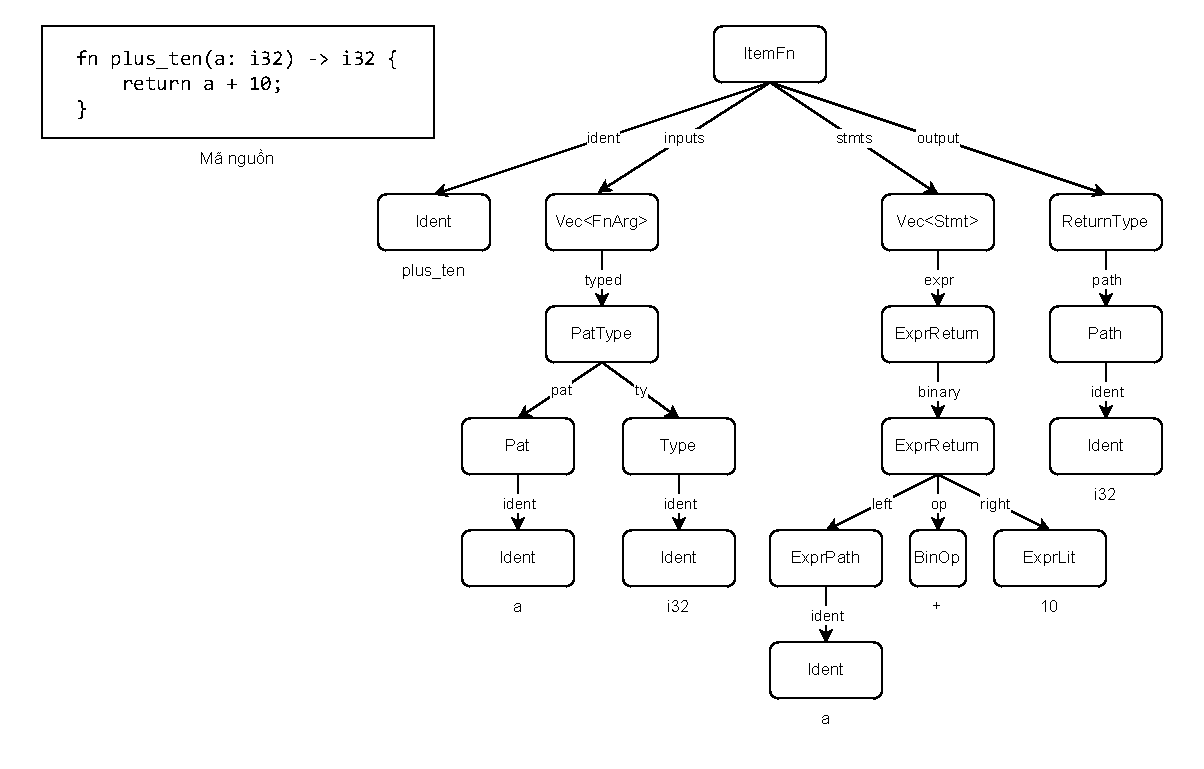
\includegraphics[width=1\columnwidth]{figures/c2/c2_ast.drawio.pdf}
  \centering
  \caption{Ví dụ về cây AST cho mã nguồn Rust.}
  \label{img:c2_ast}
\end{figure}

\subsection{Đồ thị luồng điều khiển}

Đồ thị luồng điều khiển (Control Flow Graph) \cite{yan2019classifying} là đồ thị có hướng, mô tả thứ tự thực thi của các mệnh đề và điều kiện để một mệnh đề được thực thi.
Các nút là các mệnh đề hoặc mệnh đề điều kiện, được nối với nhau bằng các cạnh có hướng, thể hiện thứ tự điều khiển giữa các nút.
Một nút là mệnh đề thì có 1 cạnh ra.
Nếu một nút là mệnh đề điều kiện thì sẽ có 2 cạnh ra, bao gồm một cạnh điều khiển khi điều kiện đúng và một cạnh điều khiển khi điều kiện sai.
CFG được sử dụng cho nhiều ứng dụng phân tích ngữ cảnh, phân tích mã độc hại \cite{gascon2013structural}, định hướng cho công cụ kiểm thử mờ \cite{sparks2007automated}.
Tuy nhiên, CFG không chứa thông tin về luồng dữ liệu, do vậy không đủ toàn diện để ứng dụng phát hiện lỗ hổng bảo mật trong mã nguồn.

\begin{figure}[H]
  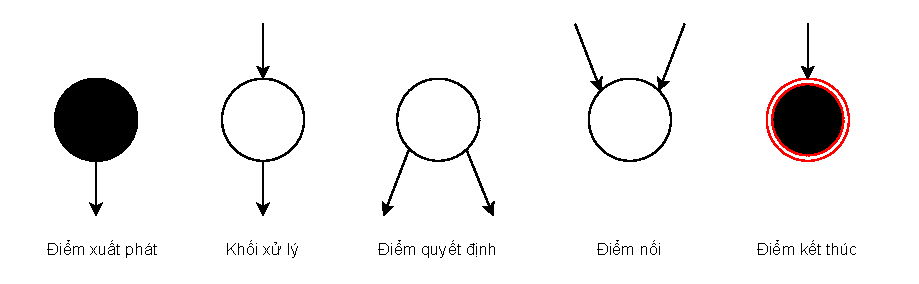
\includegraphics[width=1\columnwidth]{figures/c2/c2_cfg_point.drawio.pdf}
  \centering
  \caption{Các thành phần cơ bản trong đồ thị CFG.}
  \label{img:c2_cfg_point}
\end{figure}

Đồ thị luồng điều khiển bao gồm các thành phần chính là điểm xuất phát, khối xử lý, điểm quyết định, điểm nối và điểm kết thúc.
Trong Hình \ref{img:c2_cfg_point}, \textbf{điểm xuất phát} và \textbf{điểm kết thúc} biểu thị điểm bắt đầu và kết thúc của chương trình, lần lượt được thể hiện bằng hình tròn đặc và hình tròn đặc có viền.
\textbf{Khối xử lý} tượng trưng cho các câu lệnh gán, khai báo và khởi tạo, được thể hiện bằng hình tròn rỗng.
\textbf{Điểm quyết định} biểu thị các câu lệnh điều kiện trong các khối lệnh rẽ nhánh, được thể hiện bằng hình tròn rỗng với hai cạnh đi ra.
\textbf{Điểm nối} biểu thị các câu lệnh thực hiện ngay sau các lệnh rẽ nhánh, có hai cạnh nối đến, được thể hiện bằng hình tròn rỗng.

\begin{figure}[H]
  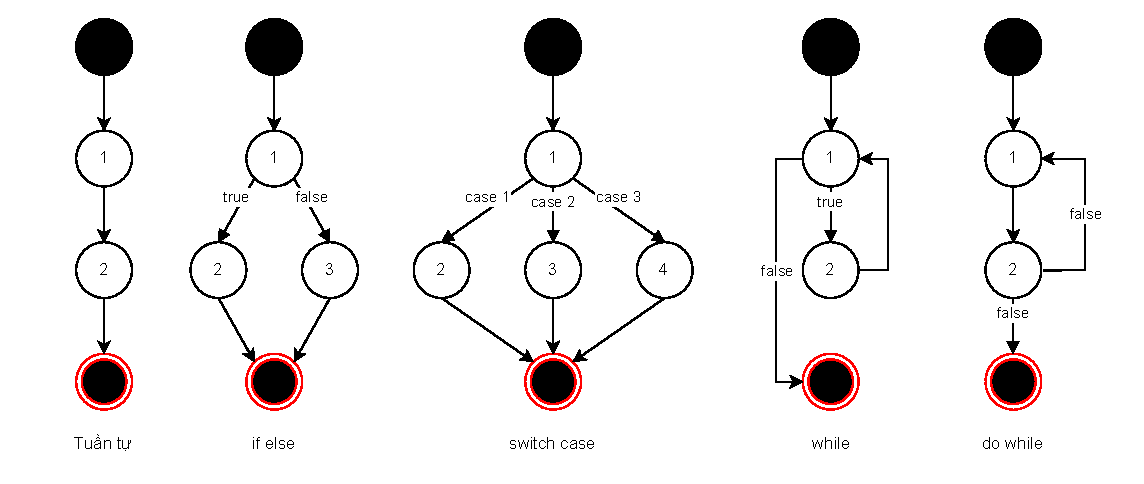
\includegraphics[width=1\columnwidth] {figures/c2/c2_cfg_line.drawio.pdf}
  \centering
  \caption{Các cấu trúc điều khiển phổ biến trong ngôn ngữ lập trình.}
  \label{img:c2_cfg_line}
\end{figure}

Hình \ref{img:c2_cfg_line} mô tả các cấu trúc điều khiển phổ biến có trong các ngôn ngữ lập trình được biểu diễn dưới dạng đồ thị CFG, bao gồm có cấu trúc điều khiển tuần tự, if else, switch case, while và do while.

\subsection{Đồ thị phụ thuộc chương trình}

% The PDG makes explicit both the data and control dependences for each operation in a program. Data dependence graphs have provided some optimizing compilers with an explicit representation of the definition-use relationships implicitly present in a source program [31, 361]. A control flow graph [1, 31] has been the usual representation for the control flow relationships of a program; the control conditions on which an operation depends can be derived from such a graph. An undesirable property of a control flow graph, however, is a fixed sequencing of operations that need not hold. The program dependence graph explicitly represents both the essential data relationships, as present in the data dependence graph, and the essential control relationships, without the unnecessary sequencing present in the control flow graph.’ These dependence relationships determine the necessary sequencing between operations, exposing potential parallelism.

% The PDG represents a program as a graph in which the nodes are statements and predicate expressions (or operators and operands) and the edges incident to a node represent both the data values on which the node’s operations depend and the control conditions on which the execution of the operations depends

Đồ thị phụ thuộc chương trình (Program Dependence Graph) \cite{ferrante1987program} là đồ thị có hướng thể hiện hai khía cạnh của chương trình, phụ thuộc điều khiển và phụ thuộc dữ liệu.
Một nút đại diện cho các mệnh đề hoặc mệnh đề điều kiện, một cạnh thể hiện mối quan hệ phụ thuộc điều khiển hoặc phụ thuộc dữ liệu giữa các nút.
Mệnh đề mà một nút đại diện có được thực thi hay không phụ thuộc vào các cạnh điều kiện điều khiển trỏ tới nút, giá trị của các biến mà mệnh đề sử dụng phụ thuộc vào các cạnh phụ thuộc dữ liệu trỏ tới nút đó.
Lưu ý rằng cạnh phụ thuộc điều khiển không giống như cạnh luồng điều khiển của đồ thị CFG.
Cạnh phụ thuộc điều khiển chỉ thể hiện điều kiện để mệnh đề của một nút được thực thi, không thể hiện thứ tự thực thi của mệnh đề giữa các nút.

\begin{figure}[H]
  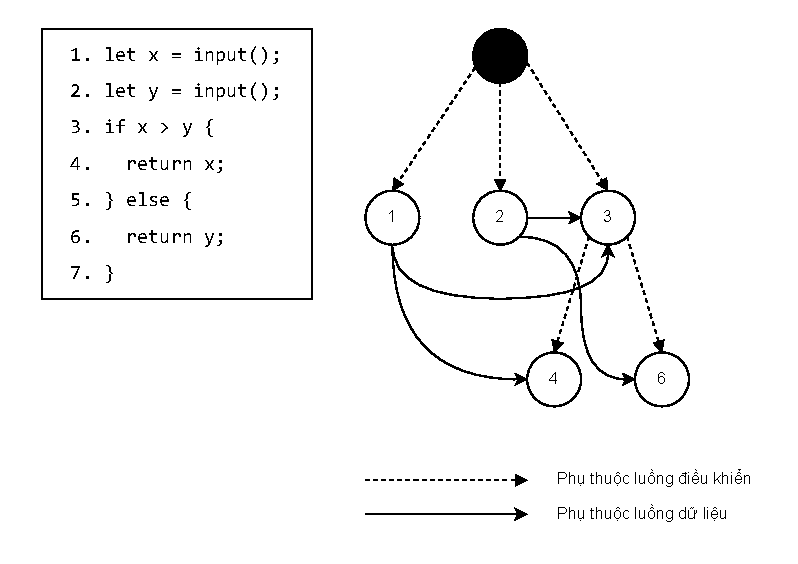
\includegraphics[width=1\columnwidth]{figures/c2/c2_pdg_3.drawio.pdf}
  \centering
  \caption{Ví dụ về đồ thị PDG.}
  \label{img:c2_pdg}
\end{figure}

Hình \ref{img:c2_pdg} biểu diễn ví dụ về một đồ thị PDG với cấu trúc điều kiện if else trong ngôn ngữ Rust, các cạnh nét đứt biểu diễn phụ thuộc điều khiển và các cạnh nét liền biểu diễn phụ thuộc dữ liệu.

\subsection{Đồ thị thuộc tính mã nguồn}

Đồ thị thuộc tính mã nguồn (Code Property Graph) \cite{yamaguchi2014modeling} là một dạng đồ thị biểu diễn mã nguồn hợp thành từ cây AST, đồ thị CFG và đồ thị PDG.
Đồ thị chứa các thông tin về cấu trúc cú pháp, luồng điều khiển và phụ thuộc dữ liệu trong chương trình
Đồ thị CPG tạo ra một lớp biểu diễn trung gian cho mã nguồn mà không bị phụ thuộc vào ngôn ngữ lập trình cụ thể.
Các nút đại diện cho các thành phần như hàm, biến, lớp và các cạnh đại diện cho mối quan hệ giữa chúng như lời gọi hàm, sự gán giá trị, quan hệ cha con hay tham chiếu.
Mỗi nút, cạnh đều có các thuộc tính, mỗi thuộc tính có giá trị riêng.
Đồ thị CPG được ứng dụng để tìm kiếm lỗ hổng trong mã nguồn, phát hiện sao chép mã nguồn bằng học máy, học tăng cường \cite{zhou2019devign, han2023bjxnet}.
Hình \ref{img:c2_cpg_yamaguchi} minh họa một đồ thị CPG cho mã nguồn C \cite{yamaguchi2014modeling}.

% \begin{figure}[H]
%   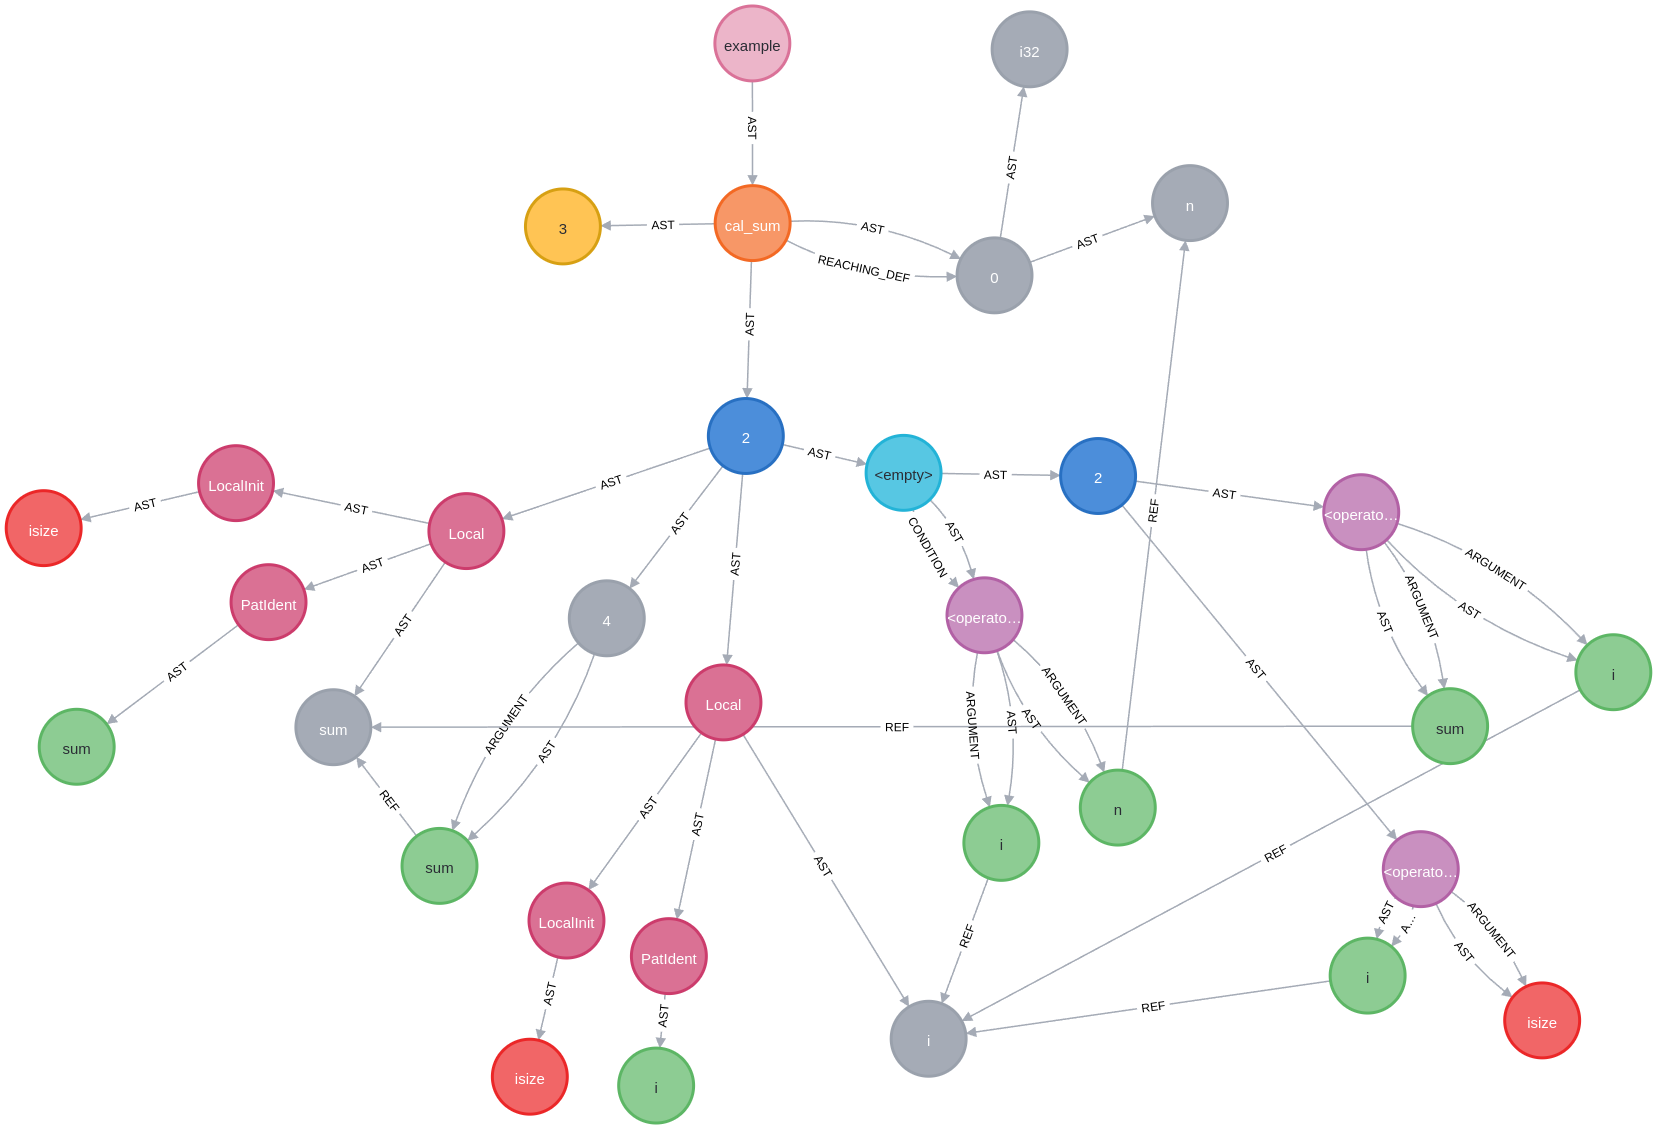
\includegraphics[width=1\columnwidth]{figures/c2/c2_cpg.png}
%   \centering
%   \caption{Minh họa đồ thị CPG.}
%   \label{img:c2_cpg}
% \end{figure}

\begin{figure}[H]
  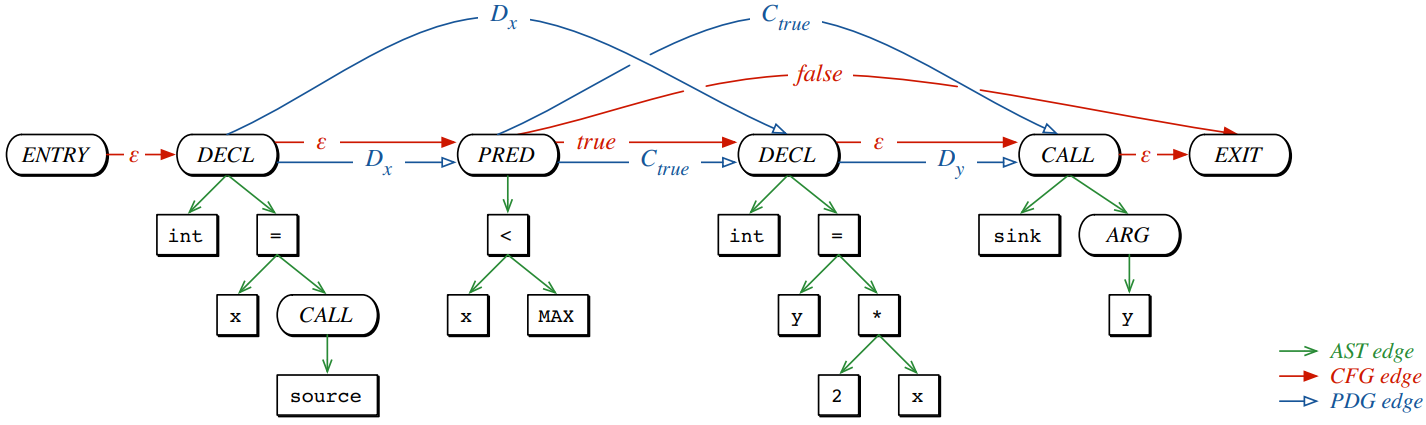
\includegraphics[width=1\columnwidth]{figures/c2/c2_cpg_yamaguchi.png}
  \centering
  \caption{Minh họa đồ thị CPG \cite{yamaguchi2014modeling}.}
  \label{img:c2_cpg_yamaguchi}
\end{figure}


% \begin{listing}[H]
% \begin{minted}[mathescape, breaklines, frame=lines, framesep=2mm, baselinestretch=1.2, fontsize=\footnotesize, linenos]{rust}
% fn cal_sum(n: i32) {
%   let mut sum = 0;
%   let mut i = 1;
%   while i <= n {
%       sum += i;
%       i += 1;
%   }
%   return sum;
% }
% \end{minted}
% \caption{Mã nguồn đầy đủ cho đồ thị CPG Hình \ref{img:c2_cpg}.}
% \label{code:c2_cpg}
% \end{listing}

\section{Công cụ Joern}

\subsection{Đặc tả đồ thị thuộc tính mã nguồn của Joern}

Đồ thị thuộc tính mã nguồn đã được nghiên cứu rộng rãi, có rất nhiều phiên bản cài đặt được xây dựng dành cho các mục đích khác nhau \cite{yamaguchi2014modeling, xiaomeng2018cpgva, kuchler2022representing, githubGitHubWimkeirgraft, githubGitHubPlumeossplume, joernJoernHunteraposs, fraunhoferaisecHomeCode, banse2021cloud, weiss2022language, keirsgieter2020graft}.
Tuy nhiên có một phiên bản mã nguồn mở được do chính tác giả của đồ thị thuộc tính mã nguồn, Fabian Yamaguchi, đích thân phát triển và duy trì có tên Joern \cite{joernJoernHunteraposs}.

Dự án CPG [6, 8] cho phép biểu diễn mã nguồn của các ngôn ngữ lập trình khác nhau dưới dạng đồ thị.
Cho đến nay, trọng tâm là Java và C/C++ nhưng hỗ trợ thử nghiệm cho Python, Go và TypeScript cũng có sẵn.
Mục tiêu của dự án là cung cấp một cách biểu diễn mã nguồn không phụ thuộc vào ngôn ngữ.
Điều này cho phép chuyên gia bảo mật xác định các lỗ hổng hoặc lỗi.
Hơn nữa, thư viện CPG bao gồm một cách để lưu trữ đồ thị trong neo4j2 và làm cho đồ thị có thể truy cập qua giao diện dòng lệnh.
Trong một số trường hợp, thư viện cũng có thể đánh giá giá trị mà một nút có thể giữ.
Tất cả những điều này cho phép chuyên gia bảo mật viết các truy vấn tùy chỉnh cho cơ sở dữ liệu đồ thị hoặc cách biểu diễn CPG trong bộ nhớ.
Thư viện CPG được thiết kế để cho phép tái sử dụng các truy vấn này giữa tất cả các ngôn ngữ lập trình được hỗ trợ.
Để đạt được mục tiêu này, thư viện CPG thực hiện một hệ thống phân cấp lớp đầy đủ, bao gồm các loại câu lệnh và biểu thức khác nhau.
CPG mã hóa thông tin như hệ thống phân cấp lớp của mã đang được phân tích, đồ thị luồng điều khiển và đồ thị cuộc gọi trong một đồ thị duy nhất.
Thiết kế hiện tại chủ yếu nhắm vào các ngôn ngữ lập trình hướng đối tượng.
Để đối phó với khả năng thiếu một số đoạn mã hoặc lỗi trong mã, thư viện có khả năng chịu lỗi với mã không đầy đủ, không biên dịch được và thậm chí ở mức độ nào đó còn không chính xác.

% Đồ thị thuộc tính mã nguồn (Code Property Graph - CPG) là một cấu trúc dữ liệu được thiết kế để khai thác các cơ sở mã nguồn lớn nhằm tìm kiếm các mẫu lập trình.
% Những mẫu này được hình thành trong một ngôn ngữ đặc thù (DSL) dựa trên Scala.
% CPG đóng vai trò như một biểu diễn chương trình trung gian duy nhất cho tất cả các ngôn ngữ được Joern và phiên bản thương mại của nó là Ocular hỗ trợ.

% Đồ thị thuộc tính là một trừu tượng chung được hỗ trợ bởi nhiều cơ sở dữ liệu đồ thị đương đại như Neo4j, OrientDB và JanusGraph.
% Trên thực tế, các phiên bản cũ của Joern đã sử dụng các cơ sở dữ liệu đồ thị mục đích chung làm nơi lưu trữ và ngôn ngữ truy vấn đồ thị Gremlin.
% Tuy nhiên, khi những hạn chế của cách tiếp cận này trở nên rõ ràng theo thời gian, chúng tôi đã thay thế cả hệ thống lưu trữ và ngôn ngữ truy vấn bằng cơ sở dữ liệu đồ thị OverflowDB của riêng mình.

Các thành phần cấu thành đồ thị thuộc tính mã nguồn bao gồm:

\begin{itemize}
  \item \textbf{Các nút và loại của chúng:} Các nút đại diện cho các thành phần của chương trình.
  Điều này bao gồm các cấu trúc ngôn ngữ cấp thấp như phương thức, biến, và cấu trúc điều khiển, cũng như các cấu trúc cấp cao hơn như điểm cuối HTTP hoặc các kết quả phân tích.
  Mỗi nút có một loại, loại này chỉ ra loại thành phần chương trình mà nút đó đại diện, ví dụ, một nút với loại METHOD đại diện cho một phương thức, trong khi một nút với loại LOCAL đại diện cho khai báo của một biến cục bộ.
  \item \textbf{Cạnh có nhãn:} Quan hệ giữa các thành phần chương trình được biểu diễn thông qua các cạnh giữa các nút tương ứng của chúng.
  Ví dụ, để biểu thị rằng một phương thức chứa một biến cục bộ, chúng ta có thể tạo một cạnh với nhãn CONTAINS từ nút của phương thức đến nút của biến cục bộ.
  Bằng cách sử dụng các cạnh có nhãn, chúng ta có thể biểu diễn nhiều loại quan hệ khác nhau trong cùng một đồ thị.
  Hơn nữa, các cạnh có hướng để biểu thị, ví dụ, rằng phương thức chứa biến cục bộ nhưng không phải ngược lại.
  Nhiều cạnh có thể tồn tại giữa cùng hai nút.
  \item \textbf{Cặp khóa-giá trị:} Các nút mang các cặp khóa-giá trị (thuộc tính), trong đó các khóa hợp lệ phụ thuộc vào loại nút.
  Ví dụ, một phương thức có ít nhất tên và chữ ký, trong khi một khai báo biến cục bộ có ít nhất tên và loại của biến được khai báo.
\end{itemize}

Tóm lại, đồ thị thuộc tính mã nguồn là các đồ thị có hướng, được gán nhãn cạnh, và chứa các thuộc tính, và chúng tôi khẳng định rằng mỗi nút mang ít nhất một thuộc tính chỉ ra loại của nó.
Điều này giúp cho việc phân tích mã nguồn trở nên dễ dàng và hiệu quả hơn, đồng thời mở ra nhiều khả năng cho việc tìm kiếm và phát hiện các mẫu lập trình trong các cơ sở mã nguồn lớn.

\begin{itemize}
  \item Đặc tả CPG của Joern được thiết kết chủ yếu cho ngôn ngữ C/C++ và Java, đưa ra các chuẩn chung như (if else, swtich case, while, for, ...) mà nhiều ngôn ngữ khác có điểm tương đồng như Python, Go, TypeScript, ... có thể tuân thủ.
  \item Tuy nhiên chuẩn chung này không thể đáp ứng được nhu cầu của tất cả các ngôn ngữ. Joern tập trung cho 2 ngôn ngữ lớn là C/C++ và Java do vậy sẽ đặc tả có sẵn (hiện có) sẽ phù hợp với các ngôn ngữ có cú pháp C-like và hướng đối tượng (OOP)
  \item Trong khi đó Rust là một ngôn ngữ lập trình mới, có cú pháp dựa trên C-Like nhưng vẫn có đôi chút sự khác biệt vì đây là ngôn ngữ hiện đại, hỗ trợ đan xen cả hướng đối tượng và hướng hàm. Đặc biệt với tính hướng hàm, Rust có nhiều cú pháp mới mà Joern chưa hỗ trợ, hay những biểu thức, mệnh đề trong C/C++ hay Java là không hợp lệ nhưng trong Rust thì hoàn toàn có thể
  \item Nhìn chung bản đặc tả CPG của Joern cung cấp 1 baseline bao phủ các tính năng phổ biến mà ngôn ngữ lập trình nào cũng có (cùng ý nghĩa nhưng có thể sử dụng cú pháp, keyword khác nhau) như $if\ else$, ... nhưng không thể đáp ứng được tất cả các ngôn ngữ lập trình hiện đại. Do vậy đối với từng ngôn ngữ riêng biệt vẫn phải bổ sung thêm các đặc tả mới cho phù hợp với từng ngôn ngữ, đặc biệt là Rust có cơ chế quản lý bộ nhớ an toàn thể hiện qua các tính năng $ownership$, $borrowing$, $lifetime$ mà Joern chưa hỗ trợ, và cả tính năng hướng hàm
\end{itemize}

\textbf{Joern Backend, Joern Frontend}

\begin{figure}[H]
  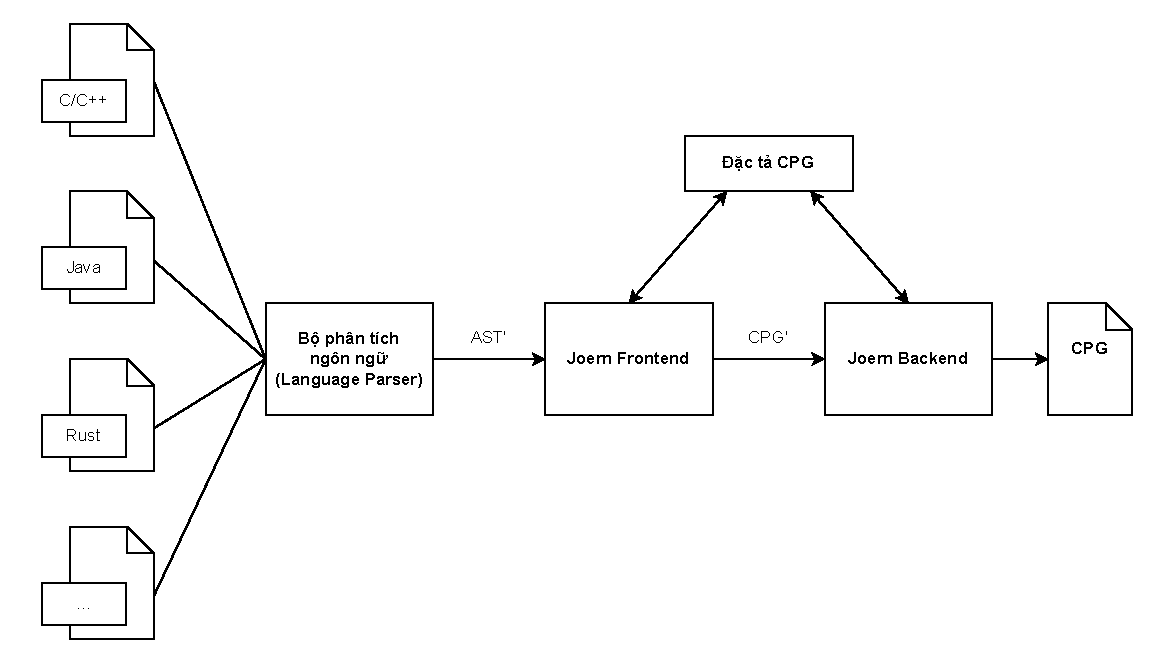
\includegraphics[width=1\columnwidth]{figures/c2/c2_frontend_backend.drawio.pdf}
  \centering
  \caption{Cách hoạt động của công cụ Joern.}
  \label{img:c2_frontend_backend}
\end{figure}

\begin{itemize}
  \item Ngoài phần đặc tả CPG dùng chung cho nhiều ngôn ngữ trên lý thuyết, Joern còn cung cấp 1 kiến trúc cài đặt thực tế có tính mở rộng cao, tương ứng với đặc tả CPG. Joern hiển tại hỗ trợ rất nhiều ngôn ngữ C/C++, Java, Python, Go, TypeScript, ... Để có thể hỗ trợ được nhiều ngôn ngữ như vậy thì Joern sử dụng 2 thành phần chính là Joern Frontend và Joern Backend, đây là 2 thành phần có tính tái sử dụng cao, không phụ thuộc vào ngôn ngữ
  \item Luồng hoạt động của kiến trúc Joern như sau. Mỗi ngôn ngữ có tập các cú pháp khác nhau, tương ứng cũng sẽ có định nghĩa về cây AST khác nhau, đây là phần người dùng muốn mở rộng Joern cho 1 ngôn ngữ mới cần phải tự đảm nhiệm. Mã nguồn của 1 ngôn ngữ sau được được công cụ Language Parser chuyển thành cây $AST*$. Cây $AST*$ ở đây không nhất thiết chỉ dừng ở đúng mức độ thông tin là 1 cây AST mà có thể bổ sung thêm thông tin khác như kiểu dữ liệu, vị trí trong mã nguồn, ... nhưng tối thiểu đảm bảo đủ thông tin là 1 cây AST tối thiểu. Ví dụ như các ngôn ngữ có sự phát triển lâu dài như C/C++ hay Java sử dụng CDT/ JDT để làm Language Parser. CDT/JDT là công cụ rất mạnh, được dùng trong các IDE nên số lượng thông tin rất đáng kể. Còn những ngôn ngữ hiện đại như Rust, Go thì các công cụ như này chưa được phát triển toàn diện nên thông tin của cây $AST*$ chưa được đầy đủ. \item Sau khi có cây $AST*$, cây này sẽ được biến đổi thành đồ thị thuộc tính mã nguồn (CPG) theo định nghĩa đặc tả CPG. Đây là công việc của Joern Frontend. Joern Frontend sẽ đọc cây $AST*$ và chuyển đổi thành đồ thị thuộc tính mã nguồn (CPG) theo đặc tả CPG. Joern Frontend đối với từng ngôn ngữ cũng là công việc cần thực hiện, do công việc thực tế cần làm là chuyển đổi cấu trúc dữ liệu của cây $AST*$ sang cấu trúc dữ liệu tương ứng của định nghĩa $CPG$. Joern Frontend đóng vai trò chuyển đổi cây $AST*$ sang cây $CPG$, $CPG$ bổ sung thông tin thành đồ thị $CPG$
  \item Sau khi được Joern Frontend xử lý, ta sẽ có được đồ thị $CPG*$ nhưng đồ thị $CPG*$ này là đồ thị không hoàn chỉnh. Để hoàn thiện được đồ thị $CPG$ thì ta cần phải sử dụng đến Joern Backend. Ở bước Joern Frontend, ta thực hiện bước chuyển đổi 1 node AST thành 1 node CPG, tạo thêm các cạnh để thể hiện các mối quan hệ giữa các node, tuy nhiên các cạnh này chưa thể hiện được đầy đủ đồ thị CPG bao gồm AST, CFG, PDG. Với cấu trúc dữ liệu CPG của Joern, ta chỉ cần định nghĩa 1 phần số cạnh, node cần thiết của đồ thị CPG, phần còn lại sẽ được Joern Backend thực hiện các thuật toán logic để có thể tự động suy diễn các mối quan hệ còn lại. Ví dụ trong cây AST có nút thể hiện vòng lặp $for$, ta chuyển thành nút $for$ của CPG kèm thêm 1 số thông tin như mệnh đề điều kiện, biến chỉ số vòng lặp (index). Joern Backend nắm được thông tin này thì có thể tự động suy diễn ra các mối quan hệ như $REACHING_DEF$ (du pair), $DOMINATOR$, $POST\ DOMINATOR$, $CONTROL\ DEPENDENCY$, $DATA\ DEPENDENCY$, $CONTROL\ FLOW$, $DATA\ FLOW$, ... từ đó tạo ra đồ thị CPG hoàn chỉnh. Chú ý CPG được cấu tạo từ 3 thành phần AST, CPG, PDG. Trong Joern thông tin của 3 thành phần này được chia thành 3 lớp, 1 đồ thị CPG được cấu tạo từ nhiều lớp trồng lên nhau, có thể sinh ra CPG chỉ có lớp AST, hoặc AST + CPG, hoặc AST + CPG + PDG. Hoàn toàn có thể mở rộng viết thêm các lớp khác nếu cần thiết, ví dụ như bổ sung 1 lớp thông tin về bảo mật, an toàn bộ nhớ, hay cụ thể trong Rust là lớp chứa thông tin $ownership$, $borrowing$, $lifetime$
  \item Sau khi toàn bộ thông tin của CPG được hoàn chỉnh dựa trên các lớp, dữ liệu CPG được xuất ra thành file binary, cấu trúc dữ liệu đồ thị. Dữ liệu này có thể được sử dụng để truy vấn thông qua các engine cơ sở dữ liệu đồ thị như neo4j, OrientDB, JanusGraph, ... hoặc có thể được sử dụng để phân tích, tìm kiếm thông qua các công cụ khác như Joern CLI, Joern Scan, Joern Slice, Joern Flow, Joern Export, Joern Vectors
\end{itemize}

\subsection{Bộ công cụ của Joern}

\begin{figure}[H]
  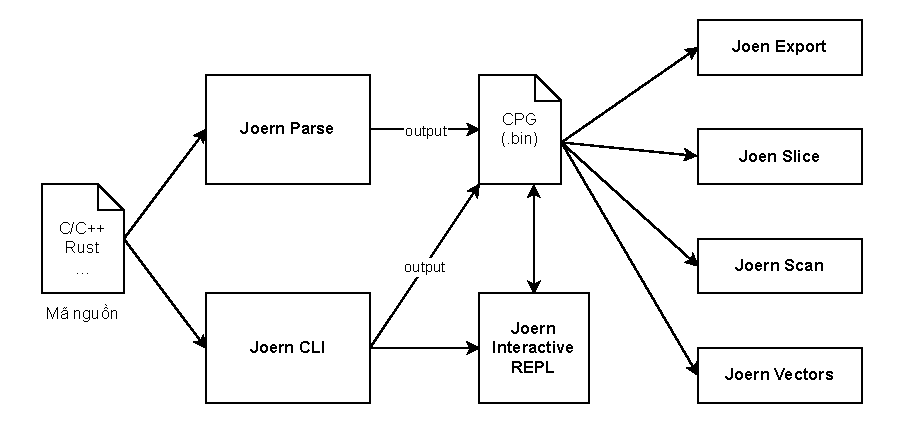
\includegraphics[width=1\columnwidth]{figures/c2/c2_joern_tools.drawio.pdf}
  \centering
  \caption{Các công cụ xung quanh Joern.}
  \label{img:c2_joern_tools}
\end{figure}

\begin{itemize}
  \item Không chỉ cung cấp kiến trúc để có thể biến đổi mã nguồn từ một ngôn ngữ sang đồ thị thuộc tính mã nguồn. Joern cần cung cấp 1 loạt các cung cấp để khai thác thông tin từ đồ thị thuộc tính mã nguồn sinh ra. Các công cụ này bao gồm: Joern Scan, Joern Slice, Joern Flow, Joern Export, Joern Vectors
  \item \textbf{JoernExport}: https://docs.joern.io/export/
  Dump intermediate graph representations (or entire graph) of code in a given export format
  Joern is used in academic research as a source for intermediate graph representations of code, particularly in machine learning and vulnerability discovery applications [e.g., 1,2,3,4,5]. To support this use-case, Joern provides both plotting capabilities in the interactive console as well as the joern-export command line utility.
  You can also export the entire graph into a neo4j csv format (along with instructions on how to import it into a running neo4j instance), graphml, graphson or graphviz dot:
  \item \textbf{JoernParse}: parse ra output ngay lập tức hoặc lưu vào cơ sở dữ liệu, không traverl
  \item \textbf{JoernSlice}: Extract various slices from the CPG.
  https://docs.joern.io/cpg-slicing/
  joern-slice is the entrypoint for Joern’s CPG slicing mechanism and specifies ways to extract useful subsets of information from the CPG. Two modes are available:
  Data-flow: This is a pretty standard backwards data-flow slicing command that starts at call arguments and slices backwards to create a graph of slices.
  Usages: This targets locals and parameters and traces what calls they make and in which calls they are used. This is useful for describing how a variable interacts in a procedure.
  \item \textbf{JoernScan}: Creates a code property graph and scans it with queries from installed bundles. QueryDB
  https://docs.joern.io/scan/
  Joern Scan ships with a default set of queries, the Joern Query Database. This set of queries is constantly updated, and contributions are highly encouraged https://github.com/joernio/joern/tree/master/querydb.
  \item \textbf{JoernVectors}: Extract vector representations of code from CPG, JoernFlow: Find flows, JoernCLI: REPL for Joern
\end{itemize}

Joern là một nền tảng mạnh mẽ dành cho việc phân tích mã nguồn, bytecode và mã nhị phân.
Công cụ này tạo ra các đồ thị thuộc tính mã nguồn (code property graphs), một cách biểu diễn đồ thị của mã giúp cho việc phân tích mã nguồn đa ngôn ngữ trở nên dễ dàng hơn.
Các đồ thị thuộc tính mã nguồn được lưu trữ trong một cơ sở dữ liệu đồ thị tùy chỉnh, cho phép khai thác mã nguồn thông qua các truy vấn tìm kiếm được xây dựng trong một ngôn ngữ truy vấn đặc thù dựa trên Scala.
Joern được phát triển với mục tiêu cung cấp một công cụ hữu ích cho việc khám phá lỗ hổng bảo mật và nghiên cứu phân tích chương trình tĩnh.

Joern hỗ trợ các nhà phát triển và nhà nghiên cứu trong việc tìm kiếm và xác định các điểm yếu tiềm ẩn trong mã nguồn, giúp nâng cao chất lượng và bảo mật của phần mềm.
Bên cạnh đó, Joern còn có khả năng phân tích mã nguồn đa ngôn ngữ, giúp các nhóm phát triển có thể làm việc với nhiều ngôn ngữ lập trình khác nhau mà không gặp trở ngại về công cụ.
Với khả năng truy vấn mạnh mẽ và linh hoạt, Joern đã trở thành một công cụ quan trọng trong việc phân tích mã nguồn và phát hiện các lỗ hổng bảo mật.
Bạn có thể tìm hiểu thêm về Joern tại địa chỉ https://joern.io/.

Joern hỗ trợ nhiều ngôn ngữ lập trình khác nhau.
Các ngôn ngữ được hỗ trợ bao gồm C/C++, Java, JavaScript, Python, x86/x64, JVM Bytecode, Kotlin, PHP, Rust, Swift, Ruby và C\#.
Điều này cho thấy Joern có khả năng phân tích mã nguồn đa ngôn ngữ, giúp các nhà phát triển và nhà nghiên cứu có thể làm việc với nhiều ngôn ngữ lập trình khác nhau mà không gặp trở ngại về công cụ.
Tuy nhiên, Joern chưa hỗ trợ cho ngôn ngữ Rust.

